%!TEX root = these.tex

\chapter{Revue de la vérification de l'exécution et des travaux connexes}

Dans ce chapitre, on revoit tout d'abord la vérification de l'exécution, y compris son histoire, sa définition et la comparaison avec d'autres techniques de vérification. D'autre part, la logique temporelle linéaire, en tant que formalisme de spécification commune de la vérification de l'exécution, est présentée avec la syntaxe, les opérateurs et la sémantique. Enfin, quelques cadres de la vérification de l'exécution bien connus sont présents, ainsi que d'une simple comparaison entre eux.

\section{Vérification de l'exécution}

La vérification et la validation de logiciels, étant considéré comme un aspect important de la gestion de projet et de l'ingénierie du logiciel, est le processus pour utiliser diverses techniques nécessaires pour détecter les violations ou les satisfactions et d'évaluer la qualité des logiciels et la performance d'un système \citep{ieeestd2012}.

\subsection{Concepts fondamentaux}

Il y a normalement deux types de techniques de vérification: analyse statique et dynamique. Certains techniques traditionnelles bien connues d'analyse statique sont la vérification de modèles \citep{clarke1999model} et la démonstration de théorèmes \citep{heisel1990tactical}. L'analyse statique est généralement appliquée pour vérifier les comportements d'un système avant son exécution, mais ces techniques ont des lacunes naturelles. Par exemple, la vérification de modèles ne peut pas fonctionner sur un système dont la taille ou le nombre d'états pourraient se développer au-delà de la capacité de puissance de calcul en raison de la ``state-explosion problem''.

L'analyse dynamique est destinée de surveiller les systèmes en cours d'exécution. Bien que parfois le résultat pourrait être de faux négatifs à cause de son incomplétude, celle-ci permet aux techniques d'analyse dynamique de briser la limitation de méthodes statiques et devenir ainsi les méthodes complémentaires de vérification. \citep{falcone2013tutorial}

la vérification de l'exécution est une sorte de technique de vérification sur la base de l'analyse dynamique. En 2001, le Runtime Verification workshop\footnote{http://www.runtime-verification.org/} a été fondée, comme la terminologie ``runtime verification'' qui a été officiellement établie \citep{wiki:rv}. Elle est une technique relativement nouvelle qui est légère et qui vise à compléter d'autres techniques traditionnelles de vérification comme ``model checking'' et ``testing''.

\cite{leucker2009brief} définissent la vérification de l'exécution comme suit:

\begin{quote}
``Runtime verification is the discipline of computer science that deals with the study, development, and application of those verification techniques that allow checking whether a run of a system under scrutiny satisfies or violates a given correctness property.''
\end{quote}

Normalement, lorsqu'une violation est observée, la vérification de l'exécution ne résout pas le programme détecté en soi, mais son résultat est un guide et une base importante pour d'autre composants dans le même système pour régler le problème.

\cite{leucker2009brief} définissent également un \emph{run} d'un système en tant qu'une séquence de traces infinies du système, et une \emph{exécution} d'un système comme une trace finie et aussi un \emph{préfixe fini} d'un \emph{run}. Le travail de la vérification de l'exécution se concentre principalement sur l'analyse d'\emph{exécutions} qui sont effectuées par les \emph{moniteurs}.

Un \emph{moniteur} est une procédure de décision générée (ou ``synthétisée'') à partir de l'une des propriétés formelles qui doit être vérifiée par rapport à l'exécution du système donné. Lors de la vérification, un \emph{moniteur} énumère les traces finies d'un \emph{exécution}, vérifie si elles satisfont aux propriétés d'exactitude et produit un \emph{verdict} comme le résultat. Un \emph{verdict}, qui est normalement une valeur de vérité, indique la satisfaction de la propriété par rapport aux événements recueillis.

Un verdict dans la plupart des cas simples peut être normalement exprimé comme vrai/faux, oui / non ou 1/0, selon le contexte. Mais en réalité, de nombreux systèmes de la vérification de l'exécution doivent introduire d'autres valeurs pour fournir un résultat plus précis. Par exemple, grâce à l'incomplétude du système de la vérification de l'exécution, un verdict ne peut pas être facilement émis lorsque le moniteur a besoin de plus d'événements successifs, donc une valeur \emph{inconcluante} (écrite comme ``?'') est introduite pour indiquer l'état présent du système surveillé. \citep{falcone2013tutorial}

\subsection{Procédure}

\begin{figure}[h]
\begin{center}
\centering
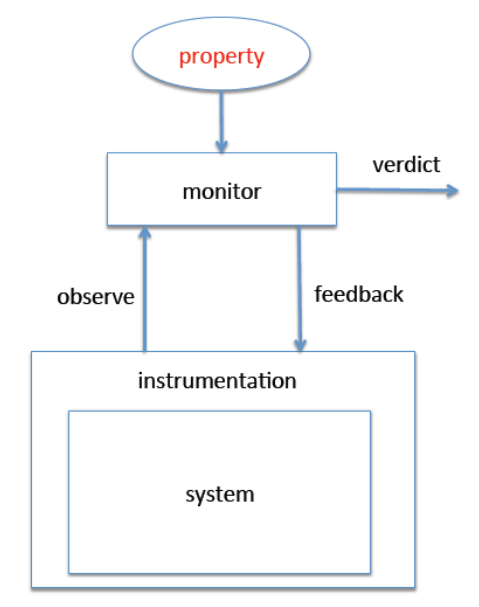
\includegraphics[width=80mm]{rvstruct.png}
\caption{Processus de la vérification de l'exécution (de \cite{falcone2013tutorial})}
\label{img:rvstruct}
\end{center}
\end{figure}

La Figure \ref{img:rvstruct} décrit le processus d'un système typique de la vérification de l'exécution qui contient les quatre étapes suivantes \citep{falcone2013tutorial}:
\begin{enumerate}
\item \emph{Synthèse du moniteur}: Un moniteur est synthétisé à partir d'une propriété.
\item \emph{Instrumentation du système}: Les instruments supplémentaires sont intégrés au système sous surveillance afin de générer les événements pour le \emph{moniteur}.
\item \emph{Exécution}: Le système est exécuté et commence à générer les événements et les envoie au moniteur.
\item \emph{Analyse et réponse}: Le moniteur analyse les événements collectés, émet un \emph{verdict} et envoie des informations supplémentaires, c.-à-d. des \emph{commentaires}, au système si nécessaire.
\end{enumerate}

Les moniteurs peuvent être classés en plusieurs modes d'aspects différents \citep{chen2007mop}:
\begin{itemize}
\item \emph{online/offline} dépend du moment où les moniteurs et le système fonctionnent: \emph{Online} s'ils travaillent en même temps, et \emph{offline} si les moniteurs commencent à travailler après la fin de l'exécution du système.
\item \emph{inline/outline} dépend de l'endroit où les moniteurs sont exécutés: \emph{Inline} si les moniteurs sont embarqués dans le système et \emph{outline} si les moniteurs fonctionnent tout seuls en recevant les traces d'événements du système par certaines méthodes, par exemple par un système de fichiers ou par un signal sans fil.
\item \emph{violation/validation} est déterminé par la spécification du verdict.
\end{itemize}

D'après les définitions des modes, on peut voir qu'un moniteur travaillant en mode \emph{offline} travaille également en mode \emph{outline} et le mode \emph{inline} implique le mode \emph{online}.

\subsection{Comparaison avec d'autres techniques}

En comparant avec la vérification de modèle \citep{clarke1999model} qui vise à vérifier les systèmes d'états finis, on voit que les méthodes de génération de moniteurs dans la vérification de l'exécution et de la génération d'automates dans la vérification de modèle ont des similitudes. Cependant, alors que la vérification de modèle traite principalement les traces infinies, la vérification de l'exécution ne traite que les traces finies, c.-à-d. les \emph{exécutions}. Pour cette raison, les moniteurs de la vérification de l'exécution travaillant en mode \emph{online} doivent être en mesure d'accepter les traces supplémentaires.

Une autre différence importante entre la vérification de modèle et la vérification de l'exécution est que, contrairement à la vérification de modèle qui vérifie si toutes les \emph{exécutions} d'un système satisfont une propriété d'exactitude, la vérification de l'exécution est intéressée uniquement par le fait qu'il y a ou non une \emph{exécution} qui appartient à un ensemble d'exécutions valides. En outre, la vérification de l'exécution requiert seulement l'analyse des événements observés d'un système donné, sans avoir à regarder ses informations internes, mais dans la vérification de modèle, le modèle approprié du système doit être reconnu afin de préparer chaque exécution possible avant l'exécution du système. \citep{leucker2009brief}

Le test du logiciel \citep{broy2005model} est une autre technique de vérification. Elle est un processus de l'exécution d'un programme avec un ensemble fini de séquences entrée-sortie qui est nommé ``la suite de tests''. En comparant avec la vérification de l'exécution, les suites de test sont définies directement, à la différence des propriétés de la vérification de l'exécution qui sont générées à partir des spécifications de formalisme. En outre, ``le test exhaustif'' qui est une méthode courante dans le test du logiciel, n'est normalement pas une option de la vérification de l'exécution.

\section{Logique Temporelle Linéaire}

Dans la vérification de l'exécution, un moniteur est traduit à partir d'une propriété d'exactitude, et les propriétés d'exactitude sont spécifiées dans les logiques temporelles en temps linéaire, telles que la logique temporelle linéaire.

La logique temporelle est une extension de la logique classique, et elle fournit un langage pratique avec les expressions des propriétés pour raisonner sur le changement des états en termes de temps. Bien qu'il y ait beaucoup de logiques temporelles différentes qui sont inventées pour satisfaire aux diverses exigences, les logiques temporelles sont normalement classées par le temps qu'il soit linéaire ou de branchement. La logique temporelle avec le temps linéaire est appelé \emph{Logique Temporelle Linéaire} (LTL), qui a d'abord été proposée par \cite{pnueli97}. le temps dans la LTL est transformé en une séquence d'états qui s'étendent vers le futur infini. La séquence d'états est un \emph{chemin} de calcul. \citep{clarke1999model,huth2004}

\cite{leucker2009brief} résument la LTL comme une logique temporelle en temps linéaire qui est bien acceptée et utilisée pour spécifier les propriétés de traces infinies. Néanmoins, dans la vérification de l'exécution, la LTL est employée pour vérifier les exécutions finies.

\subsection{Syntaxe}

Une formule LTL bien formée consiste en un ensemble fini de propositions atomiques, des opérateurs booléens $\neg, \wedge, \vee, \rightarrow$ et des opérateurs de logiques temporelles \textbf{F}(future), \textbf{G}(global), \textbf{X}(next), \textbf{U}(until), \textbf{W}(weak-until) et \textbf{R}(release). Elle peut être représentée sous la forme Backus Naur comme suit \citep{huth2004}:
\begin{align}
\phi ::= & \top | \bot | p | (\neg\phi) | (\phi \wedge \phi) | (\phi \vee \phi) | (\phi \rightarrow \phi) \nonumber \\
& | (\X \phi) | (\F \phi) | (\G \phi) | (\phi \U \phi) | (\phi \W \phi) | (\phi \R \phi)
\end{align}

\subsection{Sémantiques}

Pour une séquence d'états $s_0, s_1, s_2, ..., s_i, s_{i + 1}, ... $ où $s_{i + 1}$ est un état futur de $s_i$, on définit un chemin avec $\pi^i = s_i \rightarrow s_{i + 1} \rightarrow ... $ où $i$ est le premier état dans ce chemin. Étant donné que $\pi(i)$ est l'ensemble de propositions atomiques qui sont vraies au $i$-ème état, le fait qu'un chemin $\pi^i$ satisfait ou non une formule LTL est définie comme suit \citep{rozier2011linear}:

\begin{itemize}
  \item \listequation{\pi^i \vDash \top} \label{eq:true}
  \item \listequation{\pi^i \nvDash \bot} \label{eq:false}
  \item \listequation{\pi^i \vDash p \iff p \in \pi(i)} \label{eq:ap}
  \item \listequation{\pi^i \vDash \neg\psi \iff \pi^i \nvDash \psi} \label{eq:not}
  \item \listequation{\pi^i \vDash \psi \wedge \varphi \iff \pi^i \vDash \psi \text{ et } \pi^i \vDash \varphi} \label{eq:and}
  \item \listequation{\pi^i \vDash \psi \vee \varphi \iff \pi^i \vDash \psi \text{ ou } \pi^i \vDash \varphi} \label{eq:or}
  \item \listequation{\pi^i \vDash \psi \rightarrow \varphi \iff \pi^i \vDash \varphi \text{ chaque fois que } \pi^i \vDash \psi} \label{eq:then}
  \item \listequation{\pi^i \vDash \X \psi \iff \pi^{i + 1} \vDash \psi} \label{eq:next}
  \item \listequation{\pi^i \vDash \G \psi \iff \forall j \geq i, \pi^j \vDash \psi} \label{eq:global}
  \item \listequation{\pi^i \vDash \F \psi \iff \exists j \geq i, \pi^j \vDash \psi} \label{eq:future}
  \item \listequation{\pi^i \vDash \psi \U \varphi \iff \exists j \geq i, \pi^j \vDash \varphi$ et $\forall k, i \leq k < j, \pi^k \vDash \psi} \label{eq:until}
  \item \listequation{\pi^i \vDash \psi \W \varphi \iff$ soit $\exists j \geq i, \pi^j \vDash \varphi$ et $\forall k, i \leq k < j, \pi^k \vDash \psi$, $ \\ $soit $\forall k \geq i, \pi^k \vDash \psi} \label{eq:wuntil}
  \item \listequation{\pi^i \vDash \psi \R \varphi \iff$ soit $\exists j \geq i, \pi^j \vDash \psi$ et $\forall k, i \leq k \leq j, \pi^k \vDash \varphi$, $ \\ $soit $\forall k \geq i, \pi^k \vDash \varphi} \label{eq:release}
\end{itemize}

Les formules \ref{eq:true} et \ref{eq:false} suggèrent que les états dans le chemin $\pi^i$ devraient toujours être vrais ou faux.

Dans la formule \ref{eq:ap}, $p$ est une proposition atomique appartenant à l'ensemble fini de propositions atomiques de la LTL, et cette formule demande de vérifier seulement le $i$-ème état.

Les formules \ref{eq:not}---\ref{eq:then} sont les opérateurs booléens de la logique propositionnelle qui respectent les règles du tableau \ref{table:prologic}.

\begin{table}[h]
\centering
\begin{tabular}{|c|c|c|c|c|c|}
\hline
$\psi$ & $\varphi$ & $\neg\psi$ & $\psi \wedge \varphi$ & $\psi \vee \varphi$ & $\psi \rightarrow \varphi$ \\
\hline
Vrai & Vrai & Faux & Vrai & Vrai & Vrai \\
\hline
Vrai & Faux & Faux & Faux & Vrai & Faux \\
\hline
Faux & Vrai & Vrai & Faux & Vrai & Vrai \\
\hline
Faux & Faux & Vrai & Faux & Faux & Vrai \\
\hline
\end{tabular}
\caption{La table de vérité des opérateurs booléens de la logique propositionnelle}
\label{table:prologic}
\end{table}

Les formules \ref{eq:next}, \ref{eq:future} et \ref{eq:global} sont les conjonctions unaires de logiques temporelles . L'opérateur \X signifie ``la prochaine fois'' et il saute le $i$-ème état et évalue le chemin $\pi^{i + 1}$. L'opérateur \F signifie ``parfois dans l'avenir'' qui exige qu'à partir du $i$-ème état, une propriété reste valide dans un état futur sur le chemin. Et l'opérateur \G (``globalement'' ou ``toujours'') indique qu'une propriété devrait reste valide dans chaque état depuis la $i$-ème état jusqu'à la fin ou le futur infini.

Les formules \ref{eq:until}, \ref{eq:wuntil} et \ref{eq:release} sont les opérateurs binaires de logiques temporelles. L'opérateur\U est l'abréviation de ``until''. La formule $\psi \U \varphi$ reste valide si $\varphi$ reste valide à un état futur sur le chemin, et avant cet état, la propriété $\psi$ reste valide à chaque état. L'opérateur\W est une version faible de l'opérateur\U, sauf que pour la formule $\psi \W \varphi$, $\varphi$ n'a pas besoin de rester valide à terme dans un état futur. L'opérateur\R, qui signifie ``libérer'', est en fait une logique duale de l'opérateur\U, c.-à-d. $\psi \U \varphi \equiv \neg (\neg \psi \R \neg \varphi)$. L'opérateur\R exige que pour la formule $\psi \R \varphi$, la propriété $\varphi$ devrait continuellement rester valide jusqu'à ce que $\psi$ devienne valide et $\psi$ n'a pas besoin de rester valide à terme.

Il convient de noter que dans la LTL, les logiques à deux valeurs pourraient donner un résultat prématuré qui soit vrai ou faux. Tel que mentionné précédemment, la LTL est définie pour travailler avec les traces infinies tandis que le monitoring de la vérification de l'exécution est seulement capable de traiter les traces finies, ce qui pourrait conduire à un conflit, en particulier dans un système en cours d'exécution. Par exemple, $\F \psi$ indique que $\psi$ devraient rester valide dans un état futur. Dans un système actif, tant que $\psi$ ne reste pas valide dans les états observés, les résultats de la formule sont toujours $faux$, mais si $\psi$ devient valide dans l'observation suivante, les résultats précédents deviendront corrompus et obsolètes. Par conséquent, \cite{bauer2006monitoring} ont proposé la logique à trois valeurs (LTL$_3$) qui introduit une nouvelle valeur \emph{inconcluante} pour les cas où la propriété ne peut pas être évaluée immédiatement.

\subsection{Diverses logiques temporelles}

\subsubsection{Metric Temporal Logic}

Metric Temporal Logic (MTL) \citep{chang1994compositional} a été inventée pour raisonner sur les propriétés en temps réel. Pour préciser le temps avec exactitude, MTL coupe le temps en morceaux numérotés qui sont également appelés les modules de transition chronométrés, et emploie des opérateurs de limites pour contraindre les opérateurs de logiques temporelles. Ses formules sont définies comme suit:
\begin{align*}
\phi ::= & \bot | p | (\phi \rightarrow \phi) | (\fullmoon_{\sim{}c}\phi) | (\circleddash_{\sim{}c}\phi) | (\phi \mathrel{U}_{\sim{}c} \phi) | (\phi \mathrel{S}_{\sim{}c} \phi) \\
& \mbox{où } \sim \in \{<, =, >, \equiv_d\} \mbox{ et } c \geq 0, d \geq 2
\end{align*}

$\fullmoon_{\sim{}c}\phi$ signifie ``Suivant'', $\circleddash_{\sim{}c}\phi$ signifie ``Précédent'', $\phi \mathrel{U}_{\sim{}c} \phi$ signifie ``Jusqu'à'' et $\phi \mathrel{S}_{\sim{}c} \phi$ signifie ``Depuis'' \citep{chang1994compositional}. Étant donné que $T_i$ indique le temps du $i$-ème état du chemin $\pi^i$, le fait qu'une formule reste ou non valide à la position $j$ du chemin $\pi$ est défini comme suit (on ignore les opérateurs propositionnels ici):
\begin{eqnarray*}
\pi^i \vDash \fullmoon_{\sim{}c}\psi & \iff & \pi^{i+1} \vDash \psi \mbox{ et } T_{i+1} - T_i \sim c \\
\pi^i \vDash \circleddash_{\sim{}c}\psi & \iff & i \geq 1 \mbox{ et } \pi^{i-1} \vDash \psi \mbox{ et } T_i - T_{i-1} \sim c \\
\pi^i \vDash \psi \mathrel{U}_{\sim{}c} \varphi & \iff & \exists j \mbox{ où } i \leq j, \pi^j \vDash \varphi \\ & & \mbox{ et } T_k - T_j \sim c, et \forall k \mbox{ où } i \leq k < j, \pi^k \vDash \psi \\
\pi^i \vDash \psi \mathrel{S}_{\sim{}c} \varphi & \iff & \exists j \mbox{ où } 0 \leq j \leq i, \pi^j \vDash \varphi \\ & & \mbox{ et } T_j - T_k \sim c, et \forall k \mbox{ où } j < k \leq j, \pi^k \vDash \psi \\
\end{eqnarray*}

\subsubsection{Past Time LTL}

Considérant que dans la dernière partie la LTL est définie pour vérifier les états futurs, Past Time LTL (ptLTL) vise à vérifier les états dans le passé. Les formules de la ptLTL sont définies comme suit \citep{havelund2004efficient}:
\begin{align*}
\phi ::= & \top | \bot | p | (\neg\phi) | (\phi \wedge \phi) | (\phi \vee \phi) | (\phi \rightarrow \phi) \\
& | (\odot \phi) | (\diamond \phi) | (\boxdot \phi) | (\phi \mathrel{S_s} \phi) | (\phi \mathrel{S_w} \phi) \\
& | (\uparrow \phi) | (\downarrow \phi) | [\phi, \phi)_s | [\phi, \phi)_w
\end{align*}

Comme on le voit dans la définition de formules, la ptLTL conserve plusieurs opérateurs fondamentaux comme la LTL et introduit cinq opérateurs du temps passé et quatre opérateurs de monitoring.

Les cinq opérateurs du temps passé sont $\odot$ qui signifie ``précédent'', $\diamond$ ``finalement dans le passé'', $\boxdot$ ``toujours dans le passé'', $\mathrel{S_s}$ ``intervalle fort'' et $\mathrel{S_w}$ ``intervalle faible''.

Les opérateurs de monitoring $\uparrow \downarrow [,)_s [,)_w$ désignent respectivement ``le début'', ``la fin'', `` intervalles fort'' et ``intervalle faible''.

Les sémantiques des opérateurs temporels sont décrites comme suit, dans la même forme que la dernière section:
\begin{eqnarray*}
\pi^i \vDash \odot \psi & \iff & \mbox{ si } i > 0, \pi^{i - 1} \vDash \psi, ou \mbox{ si } i = 0, \pi^0 \vDash \psi \\
\pi^i \vDash \diamond \psi & \iff & i > 0 \mbox{ et } \exists j \mbox{ où } 0 \leq j \leq i, \pi^j \vDash \psi \\
\pi^i \vDash \boxdot \psi & \iff & i > 0 \mbox{ et } \forall j \mbox{ où } 0 \leq j \leq i, \pi^j \vDash \psi \\
\pi^i \vDash \psi \mathrel{S_s} \varphi & \iff & \exists 0 \leq j \leq i, \pi^j \vDash \varphi \mbox{ et } \forall k, j < k \leq i, \pi^k \vDash \psi \\
\pi^i \vDash \psi \mathrel{S_w} \varphi & \iff & \pi^i \vDash \psi \mathrel{S_s} \varphi \mbox{ ou } \pi^i \vDash \boxdot\psi \\
\pi^i \vDash \uparrow \psi & \iff & \pi^i \vDash \psi \mbox{ et } \pi^{i - 1} \nvDash \psi \\
\pi^i \vDash \downarrow \psi & \iff & \pi^i \nvDash \psi \mbox{ et } \pi^{i - 1} \vDash \psi \\
\pi^i \vDash [\psi, \varphi)_s & \iff & \exists j \mbox{ où } 0 \leq j \leq i, \pi^j \vDash \psi, \mbox{ et } \forall k \mbox{ où } j \leq k \leq i, \pi^k \nvDash \varphi \\
\pi^i \vDash [\psi, \varphi)_w & \iff & \pi^i \vDash [\psi, \varphi)_s \mbox{ et } \pi^i \vDash \boxdot\neg\varphi \\
\end{eqnarray*}

\subsubsection{EAGLE}

EAGLE \citep{barringer2004rule} est une logique temporelle de monitoring de traces finies supportant les équations paramétrées en combinant les sémantiques de points fixes minimales/maximales avec des opérateurs temporels.

La vérification de l'exécution en mode \emph{online} requiert l'acceptation de traces incrémentales, ce qui signifie qu'il y a des limites possibles entre les traces. Les règles de points fixes minimales/maximales ont été conçues pour résoudre ce problème. Avant d'évaluer la prochaine trace, les équations avec les règles maximales sont nécessaires pour être toujours valides et celles avec les règles minimales nécessitent seulement d'être éventuellement valides.

\section{Cadre de la vérification de l'exécution}\label{sec:rv:frameworks}

Dans la vérification de l'exécution, les moniteurs sont générés à partir de spécifications formelles par les cadres de la vérification de l'exécution. Il y a quatre modes de monitoring: \emph{offline}, \emph{online}, \emph{inline}, et \emph{outline} comme nous en avons discuté antérieurement dans cette section. De nombreux cadres et systèmes utilisant des variantes ou des extension de la LTL ont été proposés, comme le montre le Tableau \ref{table:rvframeworks}.

\begin{table}[h]
\centering
\begin{tabular}{|c|c|c|}
\hline
Non & Logique & Mode \\
\hline
JPax\citep{havelund2001java} & LTL \& Past-time LTL & outline \\
\hline
JavaMaC\citep{kim2004java} & Past-time LTL & outline \\
\hline
Hawk \citep{d2005event} & Hawk & outline \\
\hline
Temporal Rover\citep{drusinsky2000temporal} & LTL \& MTL & outline \\
\hline
MOP \citep{chen2007mop} & Divers & inline/outline/offline \\
\hline
\end{tabular}
\caption{Cadre de la vérification de l'exécution}
\label{table:rvframeworks}
\end{table}

Java PathExplorer (JPaX) \citep{havelund2001java} est un système de la vérification de l'exécution \emph{online} en vue de surveiller les traces d'exécution de programmes Java. Il dispose de trois modules (montré dans la Figure \ref{img:jpax}): un module d'instrumentation, un module d'observation et un module d'interconnexion. Le programme travaillant avec le module d'instrumentation envoie les traces nécessaires d'événements au module d'interconnexion, qui transmet ensuite les traces au module d'observation qui fonctionne éventuellement sur un autre ordinateur. Le module d'instrumentation est mis en fonction par un script spécifié par l'utilisateur en Java ou en Maude qui est destiné pour la spécification du monitoring de l'exécution.

\begin{figure}[h]
\begin{center}
\centering
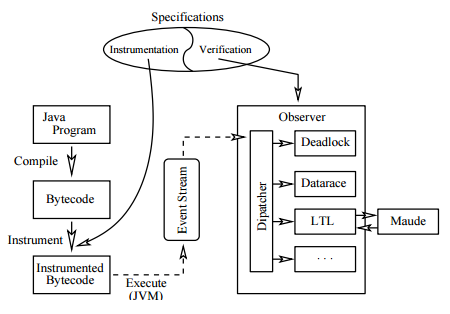
\includegraphics[width=100mm]{jpax.png}
\caption{L'architecture de JPaX \citep{havelund2001java}}
\label{img:jpax}
\end{center}
\end{figure}

JavaMaC \citep{kim2004java} est un ``système d'assurance d'exécution'' pour les programmes Java tandis que Mac signifie monitoring et vérification. Son architecture est représentée dans la Figure \ref{img:javamac}. Deux langues de définition sont proposées: l'une pour les spécifications de haut niveau qui spécifie les propriétés requises, l'autre pour la spécification de bas niveau qui définit les événements et les conditions. Pendant la préparation, un ``filtre'' et un ``reconnaisseur d'événement'' qui sont utilisés pour recueillir les traces d'événements nécessaires, sont générés à partir de la spécification de bas niveau, et un ``vérificateur d'exécution'' est généré à partir de la spécification de haut niveau. Lors de l'exécution du programme cible, les événements collectés par le ``filtre'' et le ``reconnaisseur d'événement'' sont envoyés au ``vérificateur d'exécution'' qui est alors responsable pour les travaux de la vérification de l'exécution.

\begin{figure}[h]
\begin{center}
\centering
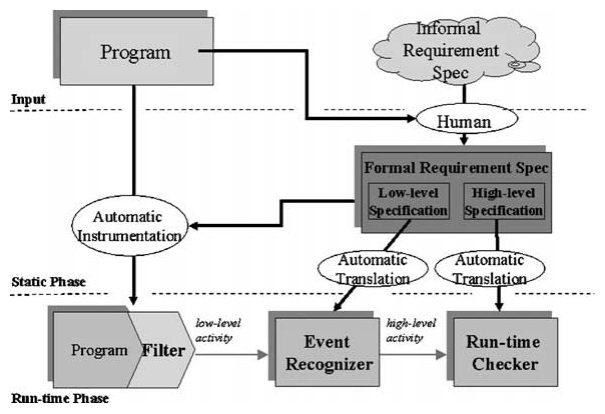
\includegraphics[width=100mm]{javamac.png}
\caption{L'architecture de MaC \citep{kim2004java}}
\label{img:javamac}
\end{center}
\end{figure}

\cite{d2005event} présentent une logique nommée HAWK et ses outils de programmes Java pour la vérification de l'exécution. HAWK est en fait construite sur EAGLE, une autre logique temporelle qui est considérée comme plus expressive \citep{barringer2004rule}. Bien que HAWK soit basée sur les événements en contraste avec EAGLE qui est basée sur les états, les spécifications de HAWK sont converties aux moniteurs d'EAGLE. Comme le décrit la Figure \ref{img:eagle}, pendant l'exécution du programme, l'état d'EAGLE est mis à jour par le programme instrumenté qui notifie alors l'observateur d'EAGLE. Après cela, l'observateur évalue la formule dans l'état actuel pour produire un résultat.

\begin{figure}[h]
\begin{center}
\centering
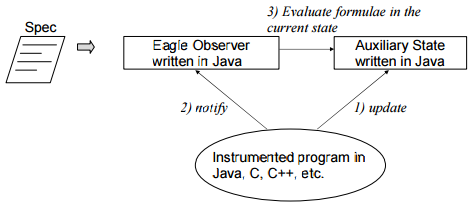
\includegraphics[width=100mm]{eagle.png}
\caption{L'architecture d'Eagle \citep{d2005event}}
\label{img:eagle}
\end{center}
\end{figure}

Temporal Rover \citep{drusinsky2000temporal} est un outil commercial de la vérification de l'exécution basé sur LTL et MTL. Le code de spécification de Temporal Rover est inséré dans le code source Java, C, C ++ ou HDL, puis converti en un fichier source compilable du langage correspondant. Un système de la vérification de l'exécution de Temporal-Rover a normalement deux parties: l'hôte et la cible. L'hôte est responsable de la vérification alors que la cible effectue le calcul de formules propositionnelles et renvoie les résultats à l'hôte via le port série, RPC ou un autre protocole configurable.

Chacun des cadres évoqués ci-dessus utilise une spécification formalisme différente, qui suggère qu'il n'existe pas une seule spécification formalisme général pouvant servir tous les objectifs. Pour être plus expressif et générique, \cite{chen2007mop} ont introduit les ``logic-plugins'' personnalisables et extensibles dans leur cadre de l'exécution MOP et ont conçu son architecture qui est représentée à la Figure \ref{img:mop} avec deux couches: l'une est appelée ``language clients'' qui soutient différents langages de programmation, tandis que l'autre est nommée ``logic repository'' qui comprend et gère divers ``logic-plugins'' pour soutenir différents formalismes de spécification, tels que: Linear Temporal Logic (LTL), Finite State Machines (FSM), Extended Regular Expressions (ERE), Context Free Grammars (CFG) and String Rewriting Systems (SRS).

\begin{figure}[h]
\begin{center}
\centering
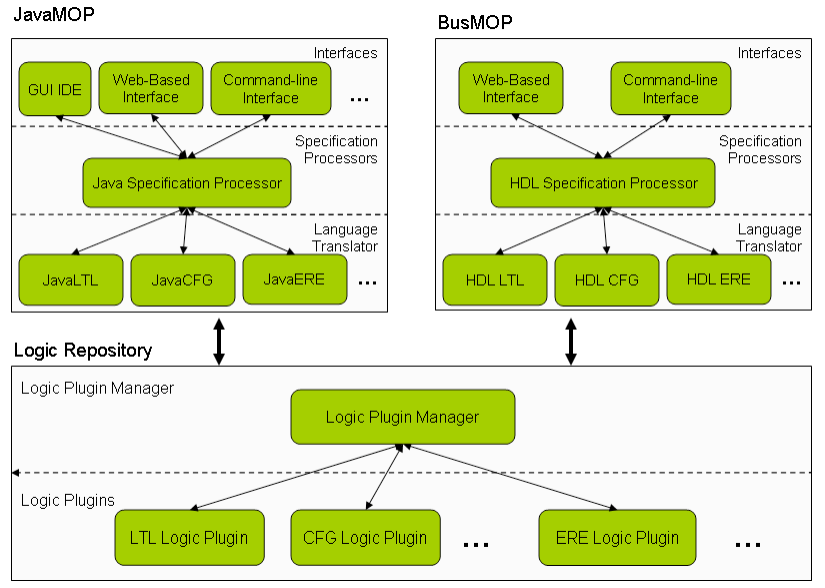
\includegraphics[width=130mm]{mop.png}
\caption{L'architecture de MOP \citep{chen2007mop}}
\label{img:mop}
\end{center}
\end{figure}

Outre les cadres présentés ci-dessus, il y a aussi beaucoup d'autres cadres inventés pour leurs exigences correspondantes ou leur logiques temporelles spécifiques. En comparant ces cadres, on peut voir qu'ils ont leurs spécialités aussi bien qu'ils partagent des caractéristiques communes. Par exemple, presque tous les cadres appuient le mode \emph{online} de monitoring, le langage de programmation Java et la communication du réseau, peut-être parce que ces caractéristiques sont les plus populaires exigées par les industries. Comme Temporal Rover est un cadre commercial, il doit donc prendre en charge plus de langages de programmation et fournir plus d'options de collecte de données pour son expansion commerciale. MOP est conçue pour être extrêmement générale, et ainsi la plupart des composants peuvent être échangés ou séparément optimisés.
